

\documentclass[twocolumn]{article}


%%%%%%%%%%%%%%%%%%%%%%%%%%%%%%%%%%%%%%%%%%%%%%%%%%%%%%%%%%%%%%%%%%%%%%%%%%%%%%%%%%%%%
% 								PACKAGE CONFIGURATION								%
%%%%%%%%%%%%%%%%%%%%%%%%%%%%%%%%%%%%%%%%%%%%%%%%%%%%%%%%%%%%%%%%%%%%%%%%%%%%%%%%%%%%%

%	For supporting accents (yep, my full name has two of them)
	\usepackage[utf8]{inputenc}
	\usepackage[T1]{fontenc}
	
%	Images
	\usepackage{graphicx}
	\fboxsep=0mm	%padding thickness
	\fboxrule=4pt	%border thickness
	\usepackage{xcolor}
	\usepackage{blindtext}

%	URLs
	\usepackage[hyphens]{url}
	\usepackage[hidelinks]{hyperref}
	\usepackage{hypcap}
	\hypersetup{breaklinks=true}
	\urlstyle{same}

%	Creating default inline TODOs
	\usepackage{blindtext}
	\usepackage[colorinlistoftodos,prependcaption]{todonotes}
	\usepackage{regexpatch}
	%\tracingxpatches%for debugging
	\makeatletter
	\xpatchcmd{\@todo}{\setkeys{todonotes}{#1}}{\setkeys{todonotes}{inline,#1}}{}{}
	\makeatother
	
%	Bibliography
	\usepackage[style=authoryear, backend=bibtex]{biblatex}
	\newcommand{\citep}[1]{\parencite{#1}}
	\addbibresource{bibliography.bib}
	\usepackage[nottoc]{tocbibind}
	\setlength\bibnamesep{2\itemsep}
	\setlength\bibitemsep{0.1\itemsep}

	
%	Colors
	\usepackage{color}
	
%	Plotting
	\usepackage{tikz}
	\usepackage{pgfplots}
	\pgfplotsset{every axis/.append style={thick}}
	
%	Counting Text with TeXCount
	%	Needs to have perl installed and in the PATH: https://www.perl.org/get.html
	%	Needs the TeXCount perl script in the PATH: http://app.uio.no/ifi/texcount/intro.html


%%%%%%%%%%%%%%%%%%%%%%%%%%%%%%%%%%%%%%%%%%%%%%%%%%%%%%%%%%%%%%%%%%%%%%%%%%%%%%%%%%%%%
% 								COMMAND CONFIGURATION								%
%%%%%%%%%%%%%%%%%%%%%%%%%%%%%%%%%%%%%%%%%%%%%%%%%%%%%%%%%%%%%%%%%%%%%%%%%%%%%%%%%%%%%

%	Setting up my new commands
\newcommand*{\ContentPath}{./content}

\newcommand{\FutureContentNotes}[1]{{\color{blue}\textbf{\textit{Notes about future content}}.- {#1}}}

\newcommand{\FutureContentNotesHidden}[1]{}






%%%%%%%%%%%%%%%%%%%%%%%%%%%%%%%%%%%%%%%%%%%%%%%%%%%%%%%%%%%%%%%%%%%%%%%%%%%%%%%%%%%%%
% 										CONTENT										%
%%%%%%%%%%%%%%%%%%%%%%%%%%%%%%%%%%%%%%%%%%%%%%%%%%%%%%%%%%%%%%%%%%%%%%%%%%%%%%%%%%%%%


\title{Quake: The Rise and Decay of the Grandfather of eSports}
\author{Rubén Osorio López}

\begin{document}

\maketitle

\begin{abstract}

This paper takes a look at why and how Quake laid the first stone in the creation of the current version of eSports to then degrade in popularity to the point that it is currently. It will examine the different reasons that caused it to be the number one competitive eSport as well as analyse how those ceased to be an advantage over time. The study will relate to events that happened in the late 90s early 2000s (1997-2001), the period that encompasses the birth of Quake as an eSport, its rise to the top and the final decline at the hands of other competitive games like \textit{Counter-Strike}.

\end{abstract}

%	Here we include all the files that contain the different sections of the document
\section{Introduction}
\label{sec::introduction}

The deafening and thunderous sound of the current eSports scene is getting more and more common each year that goes by and so is its volume as the latest The International event for Dota shows in the tremendous prize pool of almost 25 million dollars \citep{esportsEarnings}.\\

We got used to colossal games and titanic multimillion events happening every year involving eSports competitions. But every story has its beginning and this one is no different.\\

Back in the 90s when eSports as they are today could only be imagined or dreamed one game and its players started to lay the first few stones. \textbf{Quake} and its small but enthusiastic fan-base had a very significant impact in creating the foundation of the competitive gaming scene and, as such, they gained the right to be considered amongst the \textit{Grandfathers of eSports}.\\

\subsection{Defining eSport}

Before jumping into the core of the content regarding Quake it is necessary to have a common idea of what the term \textbf{eSports} means in our current context. Commonly defined as any form of competition facilitated by video-games, that definition would be slightly distant from the real meaning that it tends to have between players. When someone that knows about the eSports scene thinks about examples of what an eSport actually is games such as \textbf{\textit{League of Legends}} \citep{game:league}, \textit{\textbf{Counter-Strike}} \citep{game:cs}, \textbf{\textit{Starcraft}} \citep{game:starcraft} or \textit{\textbf{Street Fighter}} \citep{game:streetfighter} generally come to mind.\\

The common factor that these games have that the definition ignores is the fact that they all involve \textbf{direct competition} against other players. This distinction is important in the context of our topic since it leaves out of the eSports definition the competitive arcade game scene in the 80s.\\

Games such as \textbf{\textit{Pac-Man}} \citep{game:pacman} or \textbf{\textit{Donkey Kong}} \citep{game:donkeykong} had significant competition before the 90s as documented in The King of Kong \citep{kingKong}. But this type of \textbf{indirect competition} in which players try to perform better than their opponent against the machine is not very correlated to the current common eSports definition. A good argument for this is the fact that the top 100 games by prize money (softly correlated to player counts and view numbers) does not list a single game that involves \textbf{indirect competition}, all of them have a direct players versus player model.\\

Having this in mind, a good short and simple definition could be:\\

\begin{center}
\textbf{\textit{Direct video-game competitions often played for on-line or live audiences}}
\end{center}

\subsection{Introducing Quake}

Terms such as \textit{Arcade Style Shooter}, \textit{Arena-FPS} or \textit{Ego-Shooter} are commonly used to describe what Quake is. Understanding what this means is important to then being able to fully grasp why the story started and ended the way it did.\\

This game was about highly enthusiastic communities, almost reaching a somewhat healthy version of fanaticism. It came to tap into the deeply rooted but unsatisfied desire for real competition that these players had. Previously there were things such as the already mentioned arcade game tournaments but those lacked the thrill of directly defeating you opponent with your superior skills. And games such as \textit{Doom} \citep{game:doom} that offered similar game-play were significantly worse regarding the technology, availability, level of competition and more factors expanded in the next sections.\\

Here it is where the very interesting definition of \textbf{\textit{Ego-Shooter}} comes into play. Surprisingly enough, that is the translation of First-person shooter for the German language. The word \textit{Ego} here started without the usual meaning related to valuing oneself too highly but slowly morphed towards there when English speaking European players found out how well this fitted the game and its players.\\

The design of this game made it so mastery was difficult but satisfactory. This high skill ceiling is one of \textit{Quake}'s most notorious characteristics even today and it made competing against similarly passionate opponents especially attractive. Even more so than the few previous directly competitive games that came before such as the first \textit{\textbf{Street Fighter}} \citep{game:streetfighter2}.\\

\subsubsection{Why not others?}

Given that our definition already excludes indirectly competitive arcade games the only true relevant contender for the title of \textit{Grandfather of eSports} is the game that was just mentioned: \textbf{\textit{Street Fighter II}} \citep{game:streetfighter2}.\\

Two games from the \textit{Street fighter} franchise were the ones involved in the first \textit{Evolution Championship Series} in 1996. There are two main reasons why Quake's run in the late 90s makes it more relevant than \textit{Street Fighter}.\\

The first one is the raw size, visibility and quality of the first real tournament, \textbf{B3}\footnote{\textbf{B3: Battle by the Bay}\citep{evo} was the first tournament organized by the now known as \textbf{Evolution Championship Series}}. There were roughly 40 players involved and the matches were not shown on-line or to a significant live audience besides the players themselves. The only way to see some of the matches was with VHS recordings.\\

The other significant reason is that there was not another significant competition for \textit{Street fighter} until the year 2000 where another \textit{\textbf{Battle by the Bay}} tournament, the \textbf{B4}, was organized. This shows the \textbf{lack of impact} that this game had when compared to the big events that Quake had starting in 1997 with thousands of people in a live audience, high production value on-line streaming and big prize money.






\section{The History}
\label{sec::history}

\subsection{1996-1997: The Early Days}

January 1996, two young players that identified themselves on-line as "\textit{Spleenripper}" and "\textit{Dr. Rigormortis}" were already building new systems and preparing a full LAN set-up to get ready for the release of Quake \citep{clanHistory} \textbf{It was already a phenomenon} within its own niche before it was even a tangible game you could play and said release was still half a year hence.\\


The first relevant version of Quake that hit the public was \textit{QTest} \citep{qtest} on February 24, 1996. It became extremely popular amongst \textbf{players that already knew about \textit{Doom}} \citep{game:doom} and were eager to see the next big thing from \textit{id Software}. This version only could be played in multi-player, which shows the emphasis that the devs put on that aspect of the game.\\

Soon after that came the shareware edition of Quake. By this time the \textbf{formation of clans} such as \textit{The Amish}, \textit{Red Dragon} or \textit{Impulse 9} was already established in the community. The fact that these clans were astonishingly passionate about the game mixed with the gaming web boom at the time with some pages like \textit{Blue's News} hitting consistently 40.000 views a day. This created the perfect hotbed for the growth of such a new and fervent community.\\

Soon came the real deal, \textbf{the commercial release of \textit{Quake}} \citep{game:quake1} \textbf{in May 1996} only heated the circumstances. Talks about creating tournaments were being held every day at the forums and some started to happen, these were both small by current standards but big for the time. Also, the first QuakeCon \citep{quakecon} \parencite[p.~11]{van2013video} event was held in a hotel close to id Software's offices. It had 30 attendees in the first day and 100 by the end of the weekend once the news spread out.\\

\begin{figure}
	\begin{center}
		\fbox{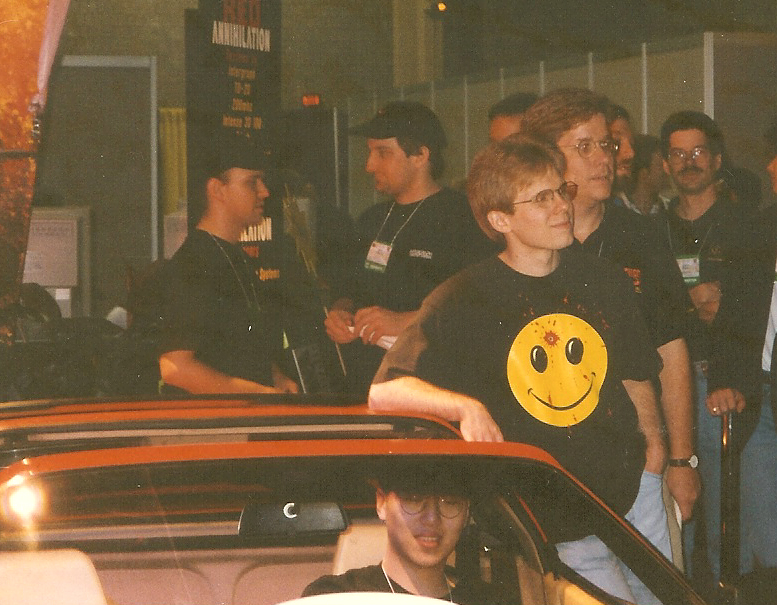
\includegraphics[width=0.95\linewidth]{resources/earlyDays.jpg}}
		
		\caption{"Thresh" wins Carmack's Ferrari. Image from \href{https://pvplive.com/c/cars-esports-prize-tournaments}{\nolinkurl{pvplive.com}}}
	\end{center}
\end{figure}

At this time nothing could compare to what happened in May of 1997 when businesses like Intergraph, Microsoft and the developers from id Software got together to organize the biggest tournament to date, they called it \textbf{\textit{Red Annihilation}s}. Said event was held during the now very famous \textbf{E3 expo} \citep{e3} in the famous \textbf{World Congress Center}.\\


This \textbf{1v1} tournament had more than 2000 participants qualifying on-line and the top 16 were flown to the live setting in the event to compete for \textbf{John D. Carmack's \footnote{John D. Carmack was the co-founder and lead developer in id Software during the era that concerns us.} Ferrari 328 GTS}. More and more breakthrough concepts kept being tied to this event. Not only the live audience was very significant but most of the spectators were able to watch the tournament via online in-game cameras professionally orchestrated. At the end of the tournament media like the NBC and The Wall Street Journal covered the event.\\

Right at that time the \textbf{CPL} \citep{web:cpl}, the pioneer in professional video-game tournament organizers, was created and a few months after, in October 1997 they organized their first event called \textbf{The FRAG} with a prize pool consisting of \$4.000 in merchandise.\\

At the end of 1997, Quake was already becoming a big hit in the gaming community and it didn't show any signs of stopping \citep{wagner2006scientific}.\\

\subsection{1998-Early 2000: Exponential growth}

\FutureContentNotesHidden{This will contain the main QuakeCon and CPL events and their growth related to the growth of eSports and the Quake community as they were.}

\textbf{\textit{Quake II}} \citep{game:quake2} was \textbf{released at the very end of 1997} and quickly became the standard for tournament play. The short intervals and significant improvements between versions of Quake had the community permanently excited to learn and compete.\\

The \textbf{year 1998} fed on the previous success and saw a significant increase in both the size of big events and the number of small ones. On July of this year, the already mentioned CPL paired with some community members involved in previous tournaments organized the third QuakeCon event, which at the same time was the second FRAG event from CPL. At the time this presented a bad view to some members of the community. Even in those circumstances, it had an attendance of 800 people and 300 BYOC \footnote{\textbf{BYOC} stands for Bring Your Own Computer, used for members of an event that carry and use their own machines.}. The prizes went from being merchandise to real money, giving \$1.000 for 5th place and scaling up to \$5.000 for first.\\

After experiencing the potential for big tournaments the \textbf{QuakeCon} dedicated more time to prepare the event without relying on the CPL. Going into the \textbf{year 1999} the event was much larger \parencite{lewis1999peace}. The major involvement from id Software as a sponsor allowed to use a much bigger venue and have developers participate. The attendance rose to 1100 people and 500 BYOC. Another important factor was the first ever tournament with \textit{Quake III} \citep{game:quake3}, which was still far from its release.\\ Later on in the year 2000, the event raised its numbers to 3000 attendees and 900 BYOC.\\

\begin{figure}
	\begin{center}
		\fbox{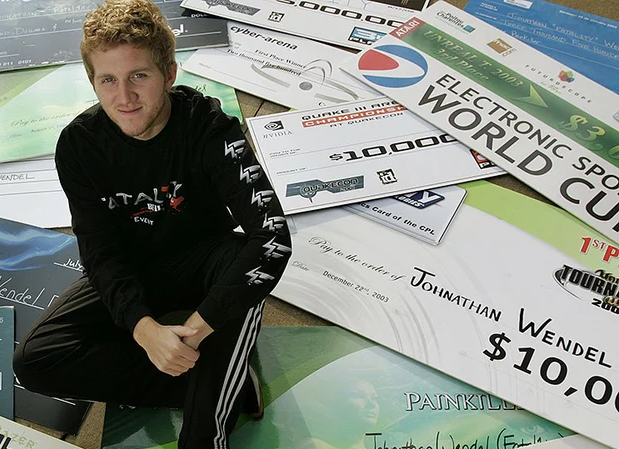
\includegraphics[width=0.95\linewidth]{resources/fatality.png}}
		
		\caption{"Fatal1ty" becoming an eSports star. Image from \href{https://www.si.com/more-sports/2016/06/30/fatal1ty-esports-professional-gaming-prize-money-motherboards}{\nolinkurl{si.com}}}
	\end{center}
\end{figure}

The \textbf{CPL} also kept blooming and establishing themselves as \textbf{the big fish in the growing pond} of eSports tournament organizers. They served as an example for many new game events and eSports leagues but none could compare to their success yet. After 1999 successful event they broke records when in the year 2000 they held a \textit{Quake III} tournament with a \textbf{prize pool of \$100.000}, 40.000 of which went to one of the rising stars of Quake, Johnathan ‘Fatal1ty’ Wendel. The existence of this characters only helped eSports and Quake to be more recognized and reach new potential fans.


\subsection{Late 2000-2001: Slayed by its own son}

\FutureContentNotesHidden{This will contain the events happened near 2001 when the main and big tournament organizers left Quake to focus on new and more liked by the public games. Mainly Counter-Strike, a game that literally came from Quake.

We can talk about how Gooseman, who worked in Quake, made the first Counter-Strike, how CS used the Quake engine as a base and how it "stole" a lot of old Quake fans and communities that naturally switches games}


\textbf{Minh "Gooseman" Le} \citep{gooseman} was a Vietnamese programmer deeply involved with the modding community of Quake. Him and another programmer in the same Quake modding team, \textbf{Jess Cliffe}, started to work on what would become the \textbf{heir of Quake} in the eSports scene, \textit{Counter-Strike} \citep{game:cs}.\\

\textit{\textbf{Counter-Strike}} came as a mod for \textit{Half-Life}, the incredibly successful First-Person Shooter game based on the \textit{Quake II} engine. Le was already used to work with said engine so modding \textit{Half-Life} felt familiar. This created a very interesting situation after the first version of the mod came in June 1999.\\

CS \footnote{CS is a common abbreviation for Counter-Strike.} kept gaining fans and getting bigger by the weeks. It was the Quake's story in a much shorter time frame. Old fans from the franchise were switching to CS, tournaments quickly put it in the same position as Quake in the year 2000 and the snowball just kept fattening and rolling down an increasingly steep hill.\\

Such was its success that \textbf{2001} saw the decline of Quake by the hands of a game that was a direct successor. Quake not only gave a large part of its technology and design to CS, but also a big part of its fan-base, Quake-based tournament and league organizers and, in general, a perfect platform for the next big eSports to grow.\\

A good example was what the CPL calls the beginning of their "\textbf{Golden Years}" \citep{web:cpl}, which at the time could be considered also the golden years of eSports given the position of the organization and the creation of the World Cyber Games \citep{WCG} \parencite[p.~28]{snavely2014history}. In 2001, the event's main title was, unsurprisingly, CS replacing the long-standing Quake. This year saw a prize-pool of \$150.000 and was regarded as the biggest event to date.\\

\textbf{The leap was immense} \citep{hope2014evolution} and so the reasons to consider Quake as the main game for a tournament or league were becoming insignificant compared to the potential wins of \textbf{having CS instead}. Other new competitive games, sometimes from other growing genres, were quickly developing and feeding from the fan-bases of older games. A good example would be \textit{Starcraft} \citep{game:starcraft} representing RTSs \footnote{\textbf{RTS} is short for the Real-Time Strategy genre or games.}.\\

In general, given the deep relationship and obsession that the core of the Quake community had with the game, id Software's franchise fell to a stable and consistent position in the shadow of the biggest, more prominent games. Looking back during the beginning of the new millennium, it looked like the years of Quake ruling the early days of the eSports kingdom were long gone \parencite{edwards2013esports}.

\section{The Reasoning}
\label{sec::reasoning}


\FutureContentNotes{
This section will be the bread and butter component of the paper. Once the right context has been set in sections \ref{sec::introduction} and \ref{sec::history} it is possible to dive deeper into the reasons that support the statement of "Quake being the Grandfather of eSports".\\

One of the subsections will focus on how the design of the game affected its situation, how those made the game very compelling at the beginning and also how those ceased to be relevant in the latter years of Quake's success. Some interesting things that will be mentioned are:

\begin{itemize}
	\item How some of the most compelling mechanics were unintended.
	\item The very steep learning curve and high skill ceiling, considered elitist by many, and its implications (not fun for casual players, the charm of the game being inherently against casual, big eSports games and players).
	\item How the good quality multi-player broke through the market allowing people to play directly against other competitors.
	\item How community creativity was very encouraged and important (Custom servers and custom maps, a lot of modding freedom with the example of Goosman, that worked on Quake and the \textit{Counter-Strike}). Now developers controll the game much more as far as eSports and who makes what content.
	\item idSoftware as a company does not keep working on the same project, they like the make, release and move on from the game model.
\end{itemize}

Another very interesting and important section will be focused on the technology of the game. So much of its success depended on how breakthrough some of the features of the games were. Some of the things worth mention would be:

\begin{itemize}
	\item Real 3D engine: Moving and looking in all axis (adding up and down compared to Doom).
	\item Best Netcode to date (TCP/IP and servers).
	\item Realistic rendering techniques performing very well in real time for the era.
	\item Lack of other games with similar technology that would impress the potential public.
\end{itemize}


Some other situational advantages that it had at the beginning could also be mentioned. A good example would be that a huge amount of people claimed that they bough Quake only for the single-player since \textit{Doom} was already a huge success years before. Then when they had already played Quake's single-player mode and discovered the multi-player it opened this door of opportunity to keep enjoying the game in a whole different way. This is important since they did not market the game for the multi-player, and people did not feel like they were gambling and buying this "new thing", they were investing in a single-player game in their eyes from a company they already trusted.\\

}

With all the different events laid out a deeper analysis of why those happened is now feasible. The reasons had to be major to justify how started from nothing and went to become this new overwhelming force in the world of gaming.\\

But perhaps what could be more interesting is how the nature of those reasons that led Quake to its top position in the year 2000 quickly turned on it and ceased to be relevant given how the community had evolved and the new games that came to take Quake's spot at the zenith.\\

\subsection{Design: Skill-based Masterpiece}

A perfect example of what Caillois defined as a game of \textit{Agon} \citep{caillois1961man}, the game was quickly categorized as a skill-dependant game which required a ton of effort to perform. The next few paragraphs will focus on how it ended up being that way and, when applicable, why those design decision, mechanics or reasons are not compelling any more.

\subsubsection{Unintended but Important}

Kicking things off on a light note there are the unplanned mechanics and the features the game had which created completely unforeseen situations.\\

\textbf{Strafe-Jumping} was a movement technique in Quake that allowed the player to jump in a certain way that would increase his velocity past the theoretical limit in the game. If players chained together these jumps and started to bounce while moving incredibly fast around the map they would be using what was called \textbf{Bunny-Hopping}.\\

Both of those features were completely unintended and came from a bug in the movement related code yet they became so deeply important that the developers left said bug intact. The significance of the mechanic was very relevant to the deeply competitive community. It had a great impact on competitive gameplay while being very hard to learn and master. Rocket-Jumping\footnote{Rocket-Jumping is a technique in which the player shoots a rocket near its feet while jumping to boost their speed and height} is another example of this.\\

But mechanics were not the only unintended but important aspect of the game. The developers fantasized at one point about having big groups and clans of people competing in their game but they themselves did not expect that to materialize nor they intended to make it happen \citep{clanHistory}. As we now know, it did in fact happen and it was what kicked things off as far as the first small eSports tournaments.

\subsubsection{Elitism, prowess and expertise}

The main defining factor for Quake which still applies today. The game had and still has an incredibly \textbf{high skill ceiling} and \textbf{massively steep learning curve} caused by the very \textbf{hard to learn mechanics}, \textbf{aim and movement focused gameplay} and the use of mainly the \textbf{1v1 mode} in the competitive scene.\\

In the \textbf{late 90s} those factors were very appealing given the potential audience. In a time where competitive gaming was so small, the only \textbf{members of the community} were ones that now would be defined as "\textit{\textbf{hardcore gamers}}" or the "\textit{tryhards}". The core of the competitive gaming community that existed at the time found a game that focused on pure skill captivating.\\

But \textbf{the more a medium grows the more of its fan-base is composed by casual followers} instead of devoted aficionados. Such often called "\textit{casuals}" in a derogatory manner by the "\textit{hardcores}" are not as interested in getting into a game that will require months or even years of practice to be able to grasp its mechanics and be a contestant.\\

Currently, a \textbf{main focus of massive competitive games is to give that fun, fast and forgiving experience} to the casual players. That allows them to amass colossal fan-bases that feed the eSports machine.\\

Quake could not be more different. The aim, movement and strategy focused gameplay and the general difficulty create this situation in which even a game with two very evenly matched players often ends in utter and complete domination. A \textbf{hugely unbalanced final score} in this game does not mean that one player is significantly better, the \textbf{skill gap might actually be minimal}. Given this situation, imagine how \textbf{crushing} games can be to a new casual player who tries to compete with the old Quake veteran, the \textbf{experience would be demolishing}.\\

\begin{figure}
\begin{tikzpicture}
  	\begin{axis}[
  		legend pos=north west,
  		legend style = {font=\footnotesize},
		xmin=-1.3,xmax=1.3,
		ymin=-1.3,ymax=1.3,
		axis lines=center,
		axis line style=-,
		ticks=none,
		%y axis line style= { draw opacity=0 },
		%xticklabels={,,}
		x label style={at={(axis description cs:1.05,0.35)},anchor=east,rotate=270},
		y label style={at={(axis description cs:0.5,1.1)},anchor=north},
		xlabel={Skill Gap},
		ylabel={Win Probability}]
		domain=-1:1]
		\legend{Quake, Casual games}
		\addplot[-,red, very thick] expression[domain=0:1, samples=100]{ 	(1-e^(-12*x))		} node[color=black,above,pos=1] {Player A}; 
		\addplot[-,blue,very thick] expression[domain=0:1, samples=100]{ 	(1-e^(-3*x))		}; 
		\addplot[-,red, very thick] expression[domain=-1:0, samples=100]{	(e^(12*x))-1		} node[color=black,below,pos=0] {Player B}; 
		\addplot[-,blue,very thick] expression[domain=-1:0, samples=100]{	(e^(3*x))-1			}; 
  	\end{axis}
\end{tikzpicture}
  	\caption{Skill Gap to Win Probability relation}
	\label{fig:skillwin}
\end{figure}

This is explained in the \textbf{Figure \ref{fig:skillwin}} which co-relates the probability that one player might win to the difference in skill between them. Values to the \textbf{top or to the right} indicate \textbf{positive or advantageous values for Player A}, when considering values to the \textbf{bottom or left} they are \textbf{positive or advantageous for Player B}.\\

If the \textbf{Skill Gap (in the X axis)} is on Player A's side in a casual game (blue line) he has indeed a higher \textbf{Probability of winning (in the Y axis)} than loosing but this probability is much higher in Quake than in some other casual game. The red line shows how even when minimal skill gaps, the win probability of the slightly better player spikes way faster in Quake compared to casual games. This creates the situation explained previously where very unbalanced scores are very common between similar players in Quake but not as common in casual games.\\

Some reasons for this have already been mentioned, such as the difficulty curve. But he fact that the biggest eSports titles are \textbf{team based} is not by chance. A team game naturally softens that spike we see in Figure \ref{fig:skillwin}'s red line. Having more people playing for a side adds more random elements that could help swing the game in favour of the team with a bad player. Such bad player in a skill-based 1v1 game is likely to loose many more games than in a team-based title.\\

There are more elements that matter, such as the in-game random elements of some competitive games. Card games are a good example of this. In \textit{Hearthstone} \citep{game:hs} a player can match up with a competitor more skilled than himself and still win because of inherently random factors such as having a deck that is very good against the opponent's, getting better cards each turn while the opponent gets bad ones or a ton of random effects that the cards in that game originate.\\

There is a famous anecdote within Quake forums in which a friend of an old Quake veteran went to his house and played the game for the first time while his friend finished some other tasks. When said veteran came back the casual player had a mixed opinion about the game, he liked the mechanics but he asked the infamous question:

\begin{quote}
\begin{center}
\textit{\textbf{Why can't I compete?}}
\end{center}
\end{quote}

Although he understood that winning should not be plausible for him he could not wrap his head around being utterly dismantled while not being able to even get a single kill even when he, as a beginner, was playing against Quake veterans that had put thousands of hours into the game. This exemplifies the elitism of Quake. If you go into a game against the top Quake player in the world you are likely to not get a single kill, in that very same case in \textit{Counter-Strike} or \textit{League or Legends} your team or you might even kill him a few times or even get the win or some rounds in the case of CS.\\

Rolling the dice and splitting responsibilities help casual players enjoy a game before they are good at it and competitive Quake follows a completely opposite philosophy with its lack of random elements, skill based gameplay and 1v1 mode.\\ 


\subsection{Technology: Engineering Gem }



\subsection{Situational}


































\section{Conclusion}
\label{sec:conclusion}

Much in the same way that the first computers, cars, televisions, movies or websites were pioneers and \textbf{disappeared from the public's mind}, Quake has suffered his own version of such fate. The very \textbf{first trailblazers} of a new medium or paradigm \textbf{are inherently modest} and concealed for the big masses. Nonetheless, that is \textbf{not a valid excuse to disregard their importance}. Be that as it may, there is a good chance that even new "\textit{hardcores}" coming into the world of eSports will not hear about Quake whatsoever.\\

Additionally, after considering everything contained in the previous sections, it is clear that \textbf{a pure Quake-Style game will not reign on top of the eSports behemoth again}. Such feat was only possible when eSports were more like a sprouting movement and not the gargantuan leviathan they are today.\\

As it happens with every growing type of media, \textbf{best and biggest tend to quickly diverge} as its popularity grows. Wolfgang Amadeus Mozart could be both the best and most popular musician in the XVIII century but if one tries to imply that the same could happen in the XXI century, Bruno Mars or Taylor Swift would beg to differ.\\

Striving to \textbf{make a popular eSports game} that is casual and sponsor-friendly is now a science and \textbf{affects videogames' design}. The final version will most usually \textbf{drastically change} if the intention was to make the \textbf{fairest, challenging and skilful product}. In defiance of such trend, Quake fans shall not be distressed. Their game, and others akin to the latter \textbf{will always have their place}. Fervent communities, although small, will continue to sustain them by reason of \textbf{the massive reward} of breaking their barrier to entry obtained in the form of even-handed entertainment, competitive enjoyment and vast sense of accomplishment.\\


%	And Here we have the bibliography citations
%	NOTE: Use \citep{id} to cite.
\nocite{*} % Used to cite everything


\printbibliography[title={Bibliography},nottype=software] 
\printbibliography[title={Videogames},type=software]

%	Our In-Progress management things
%		\listoftodos
%		\todo{Remove the TODO list}

\end{document}







%
%	Useful build command to build and copy the pdf to another folder besides /src
%	It's probably for the best to restore the build commands to default before adding and using this one
%
%	txs:///pdflatex | xcopy .\*.pdf ..\pdf /sy
%